\documentclass[titlepage]{scrartcl}
\usepackage{enumitem}
\usepackage[british]{babel}
\usepackage[style=apa, backend=biber]{biblatex}
\DeclareLanguageMapping{british}{british-apa}
\usepackage{url}
\usepackage{float}
\restylefloat{table}
\usepackage{perpage}
\MakePerPage{footnote}
\usepackage{abstract}
\usepackage{graphicx}
% Create hyperlinks in bibliography
\usepackage{hyperref}
\usepackage{amsmath}

\usepackage[T1]{fontenc}
\usepackage[utf8]{inputenc}
\usepackage{blindtext}
\setkomafont{disposition}{\normalfont\bfseries}


\graphicspath{
    {./resources/},
}
\addbibresource{~/PerryPerrySource/LaTeX/ExperimentalMusic_Bibliography.bib}

\newsavebox{\abstractbox}
\renewenvironment{abstract}
  {\begin{lrbox}{0}\begin{minipage}{\textwidth}
   \begin{center}\normalfont\sectfont\abstractname\end{center}\quotation}
  {\endquotation\end{minipage}\end{lrbox}%
   \global\setbox\abstractbox=\box0 }

\usepackage{etoolbox}
\makeatletter
\expandafter\patchcmd\csname\string\maketitle\endcsname
  {\vskip\z@\@plus3fill}
  {\vskip\z@\@plus2fill\box\abstractbox\vskip\z@\@plus1fill}
  {}{}
\makeatother

\DeclareCiteCommand{\citeyearpar}
    {}
    {\mkbibparens{\bibhyperref{\printdate}}}
    {\multicitedelim}
    {}

\begin{document}
    \title{Experimental Music\\Summative Assignment 2\\Essay}
    \subtitle{\LARGE{The role of electronic feedback and amplification in
    experimental music composition.}}
    \author{Sam Perry\\U1265119}
    \date{}

    \begin{abstract} 
        The use of electronic feedback as tools for musical composition has
        featured in many composition, popular for it's volatile and
        indeterminate nature.  Intrinsic to the use of feedback is the use of
        amplification, capable of artificially altering an input's energy, as a
        method for feedback control. This essay aims to provide a definition of
        these tools in their different forms, and to analyse their use in a
        range of prominent compositions. Forms of feedback will be defined,
        followed by a discussion of the musical implications of their use,
        including consideration for aspects such as process, indeterminacy,
        spectral implications and rhythmic implications. This will be related
        to a number of compositions in order to provide an overall
        understanding of their role in experimental music composition.
    \end{abstract}

    \maketitle

    \section{Defining feedback and amplification}
    A simple definition of feedback is the process of routing the output of a
    system back to the input of that system.~\parencite[p.1]{weisert2010ioi}
    This can take many form in the context of music, whether it is the acoustic
    feedback created by aiming a microphone to it's amplifier, or the digital
    feedback present in an IIR filter, in all cases a loop is created from an
    output point of a system, back to it's input.\\
    The three types of feedback to be considered are:
    \begin{itemize}
        \item{Acoustic Feedback}
        \item{Electronic Feedback}
        \item{Mathmatical Feedback}
    \end{itemize}
    In order to fully understand feedback, electronic amplification will also
    be explored due to it's integral part in feedback system control.
        
    \subsection{Acoustic Feedback}
    Acoustic feedback occurs when a closed loop is created between an audio
    transducer (such as a microphone or guitar pickup) and amplifier,
    causing previously amplified audio to be reamplified continuously at an
    exponential rate as illustrated in Figure~\ref{acoustic_feedback}.\\
    \begin{figure}[H]
        \makebox[\textwidth]{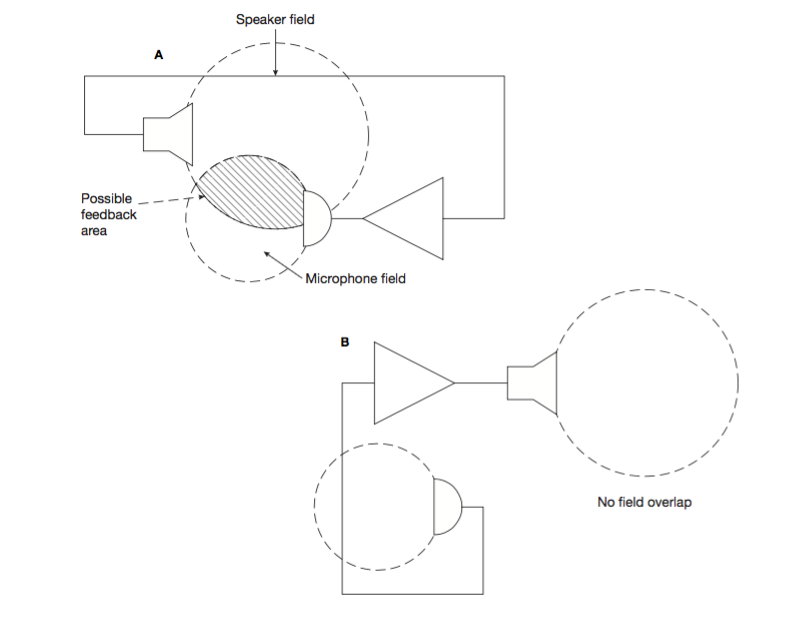
\includegraphics[width=\textwidth]{acoustic_feedback_diagram}}
        \caption[Caption for LOF]{Acoustic Feedback Diagram\protect\footnotemark}
        \label{acoustic_feedback}
    \end{figure}

    \footnotetext{Diagram taken from:~\parencite[p.185]{holmes2012eaem}}

    This is a common problem in the context of live audio, as the exponential
    nature of the feedback causes a distinct "howling" sound that builds
    rapidly and is commonly considered unplesant. As a result, a great deal of
    research has been carried out into methods for attenuating and controlling
    this effect.~\parencite[p.1]{} However, the volatile and unpredictable
    nature of acoustic feedback has been used to great effect in both popular
    and avant-garde music.  Pioneering guitarists such as Jimi Hendrix have
    used the loop created through placing an electric guitar pickup close to
    it's amplifier to compliment virtuosic guitar solos in pieces such as Foxy
    Lady~\citeyearpar{} This is taken one step further in avante-garde works
    such as Steve Reich's Pendulum Music, where feedback becomes the focus of
    the piece entirely. This is discussed further in section~\ref{pendulum}
    
    \subsection{Electronic Feedback}
    Electronic feedback takes the principal of recursively feeding an output
    back into an input into the analog electronics domain. In this situation,
    the recursive processing is performed purely on electrical signals,
    replacing the initial acoustic input from the microphone found in acoustic
    feedback, with a purely electronic input as part of an electronic circuit.
    The result of this process is then produced in the listening space via
    amplification~\parencite[p.187]{holmes2012eaem}. Composers such as David
    Tudor and Gordon Mumma explore these techniques through their creation and
    use of custom electronic circuits designed to exploit the characteristics
    of this effect.~\parencite[p.186, 390]{holmes2012eaem} A detailed analysis
    of these techniques are presented in section~\ref{ElecFeed}\\

    Although it is outside the scope of this essay, it is worth noting that
    delay feedback forms the basis for electronic IIR filtering, both in the
    analog and digital domain, and by extension is an integral part of almost
    any composition that utilises audio
    filters/equalizers.~\parencite[p.71-72]{zolzer2011dafx} This is an example
    of how the precice control of electronic feedback can lead to a plethora of
    creative musical possibilities.

    \subsection{Amplification}
    Amplification is the process of scaling a signal by a chosen factor.
    Factors $>1.$ result in an increased overall amplitude, whilst factors
    $<1.$ result in an attenuated signal amplitude~\parencite[p.3-4]{kadis2012sosr}. 
    This artificial modification of amplitude has a number of interesting sonic
    effects in itself, as it allows for the magnification of sounds that may not
    naturally be perceivable and conversely, the reduction of extremely loud
    sounds, to with a comfortable range for hearing. This explored through
    works such as John Cage's Cartridge Music and Stockhausen's Mikrophonie as
    discussed in section~\ref{amp}\\

    It has been stated that feedback (particularly acoustic feedback) is
    difficult to control. This is due to it's recursive nature and the tendancy
    in many situations for output that exceeds unity gain (a state, whereby the
    output amplitude of a feedback system is equal to that of it's input) to be
    fed back into the system. Amplification is therefor a crucial element for
    controlling the results of a feedback system. By attenuating an output
    before feeding it back to a system, it is possible to ensure that outputs
    do not grow at an exponential rate.
    \begin{figure}[H]
        \makebox[\textwidth]{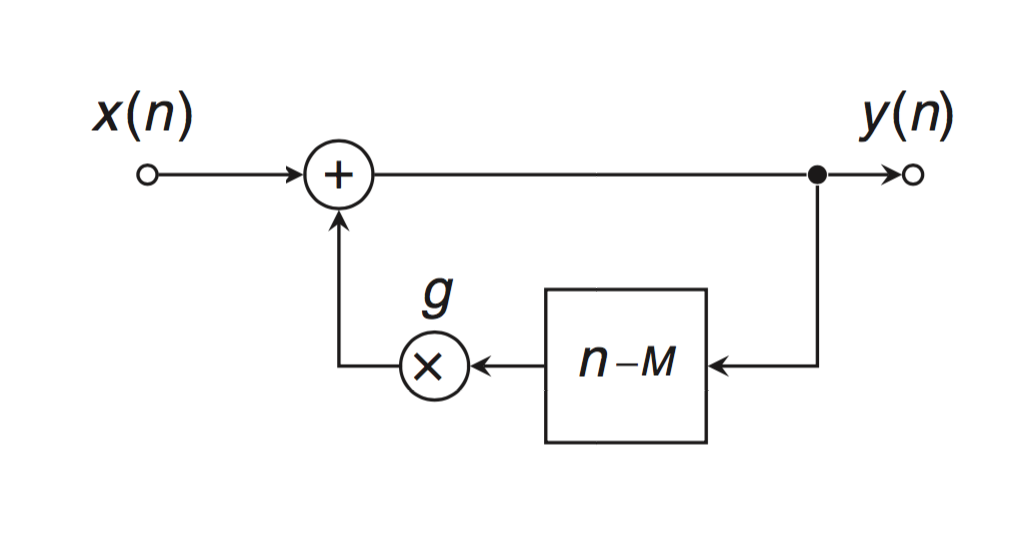
\includegraphics[width=0.75\textwidth]{IIR_flow_diagram}}
        \caption[Caption for LOF]{Basic Feedback Signal Flowchart\protect\footnotemark}
        \label{feed_flowchart}
    \end{figure}

    \footnotetext{Diagram adapted from:~\parencite[p.72]{zolzer2011dafx}}

    \begin{figure}[H]
    This can be demonstrated mathmatically using the following equation as
    illustrated in figure~\ref{feed_flowchart}:
        \begin{align*}
            & y(n) = x(n) + gy(n-M)\\
            & \text{where:}\\
            & x\text{ is the input signal}\\
            & y\text{ is the output signal}\\
            & n\text{ is the current point in time}\\
            & M\text{ is the signal delay in time}\\
            & g\text{ is the feedback coefficient}\\
        \end{align*}
    \end{figure}
    It is clear that $|g|$ dictates the stability of the signal, as values
    $>1.$ increase exponentially as stated above.~\parencite[p.70-72]{zolzer2011dafx} 

    For example, in the case of acoustic feedback, $g$ is dictated by the
    amount of signal that passes from the amplifier back to the microphone.
    Placing the microphone close will result in a large amount of the amplified
    signal returning to the amplifier, causing further amplification. When the
    system reaches it's limit (which it will do very quickly) the signal
    distorts, causing the typical "howling" effect.

    \subsection{Mathmatical Feedback}
    Rational Melody XXI - Tom Johnson
    Not electronic feedback, but serves as an example that feedback is not
    limited to electronics.
    IIR filter example?

    \section{Musical Aspects and Implications of Feedback Systems}
    \subsection{Indeterminacy}
    \subsection{Process and Control}
    \subsection{Rhythmic/Temporal Implications of Feedback}
    \subsection{Spectral Implications of Feedback}
    \subsection{Dynamic Implications of Artificial Amplitude Adjustment}

    \section{Composition Analysis}
    \subsection{Acoustic Feedback}
    \subsubsection{Steve Reich's Pendulum Music}\label{pendulum}
    \subsubsection{Robert Ashley's The Wolfman}\label{wolfman}
    - ref: kyle gann - robert ashley

    \subsection{Electronic Feedback}\label{ElecFeed}
        David Tutor's Untitled (1996), Toneburst (2004), and Pulsers (1996)
        Gordon Mumma's Hornpipe

        \subsection{Amplification}\label{amp}

    \section{Conclusion}

    \printbibliography

\end{document}
